\section{Integrationstest software}
Til udførelse af integrationstest af softwaren til systemet er det benytte sandwich testing. Dvs der er benytte nogle forskellige testing teknikker, så som buttom-up, top-down og collaboration test. \\
I inegrationstest fasen er klasserne i systemet samlet så de samlet udgøre en give funktionalitet til systemet og derved er de testet i samarbejde med hinanden.

\textbf{Top-Down/Button-Up}\\
Disse test metoder er gradvist blevet benyttet til at teste systemet. På figur \ref{fig:buttom-up} ses et eksempel på buttom up testing, her bliver systemets mest grundlæggende klasser testet og derefter bliver der testet op igennem systemet. På figur \ref{fig:top-down} ses et eksempel på top down testing, her bliver systemets top klasser testet først og derefter bliver systemet testet ned igennem klasserne.

\begin{figure}[ht]
\centering
\begin{minipage}[b]{0.45\linewidth}
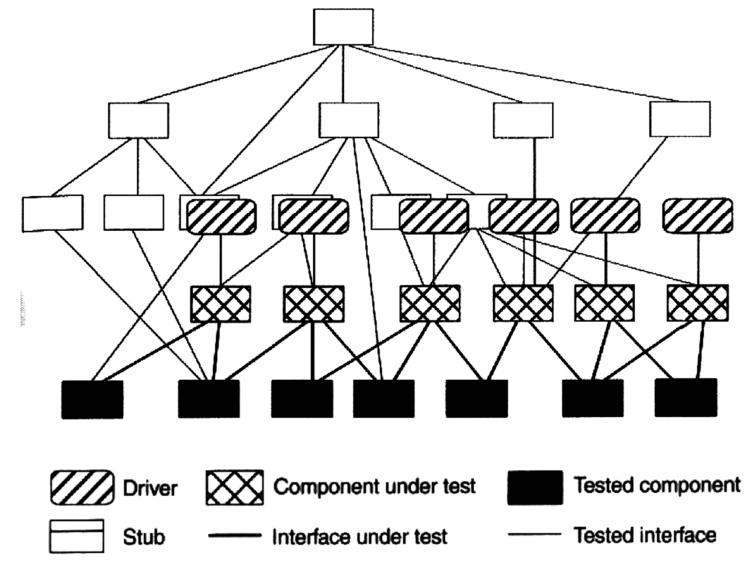
\includegraphics[width=5cm]{Billeder/Test/buttom-up.png}
\caption{Buttom-up eksempel}
\label{fig:buttom-up}
\end{minipage}
\quad
\begin{minipage}[b]{0.45\linewidth}
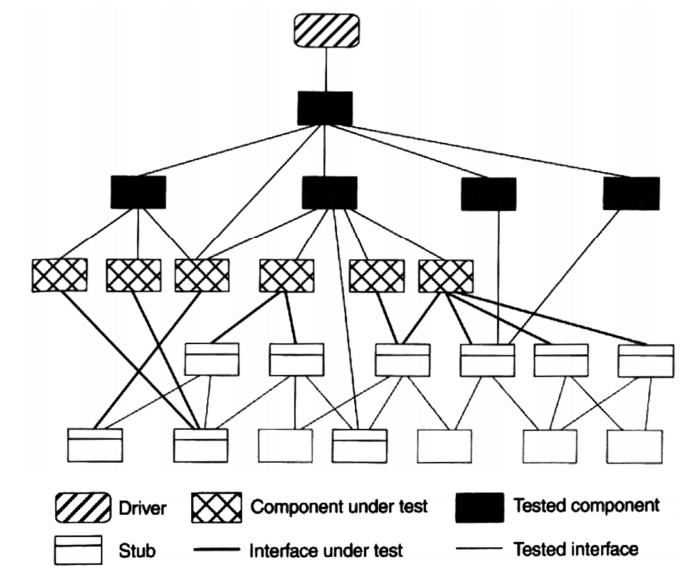
\includegraphics[width=5cm]{Billeder/Test/top-down.png}
\caption{Top-down eksempel}
\label{fig:top-down}
\end{minipage}
\end{figure}
\vspace{2cm}

\textbf{Collaboration}\\
Denne metode er blevet benytte en del under udviklings forløbet. På figur \ref{fig:Collaboration} ses et eksempel på collaboration test metoden, her samles nogle klasser i systemet så de udgøre en funktionalitet i systemet og der efter bliver klasserne testet.

\vspace{-5pt}
%kommentar
\begin{figure}[H]
	\centering
	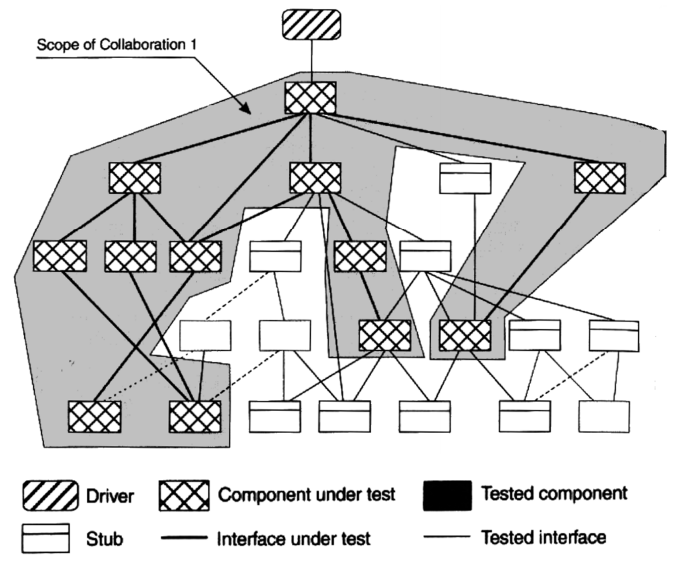
\includegraphics[width=0.5\textwidth]{Billeder/Test/collaboration.png}
	\vspace{-5pt}
	\caption{Collaboration eksempel}
	\label{fig:Collaboration}
\end{figure}